
Before we present our skyline computation algorithm in the next
section, in this section how the index and data are allocated on
the broadcast channel to form the broadcast program. We introduce
depth-first distributed-index (DFDI), our index allocation
technique, that is based on the distributed index allocation
proposed in \cite{data_on_air}. The benefits of a distributed
index over other allocation methods has been discussed in section
\ref{sec:wireless_bcast_index}.

We utilize an R-Tree~\cite{DBLP:conf/sigmod/Guttman84} to index our
multi-dimensional data records. We assume that each node of an R-Tree
consists of $b$ number of entries, $\{E_1, E_2, ... E_b\}$, where
$b$ is the branching factor, or the number of children at each internal
node, of the index tree, as illustrated by Figure~\ref{fig:index_node}.
Each entry contains a pointer to a child index node, if the node is not
a leaf node, or a pointer to a set of data records, if the node is a leaf
node. The pointer is the time when the child item will appear on the
broadcast channel.

In addition, each entry contains an orthotope, or a $n$-dimensional minimal
bounding rectangle (MBR), that denote the extend of the child object pointed
by the pointer of the entry (see Figure~\ref{fig:index_node}). Each
rectangle $MBR$ is defined by two opposite corners, $MBR.min$ and $MBR.max$,
also known as the ``lower-left" and ``upper-right" corners of the rectangle.
$min = (min_1, min_2, ..., min_n)$ and $max = (max_1, max_2, ..., max_n)$
are $n$-dimensional points containing minimal and maximal value of each
attribute in the rectangle, respectively. In other words, $min_i$ is the
lower bound, and $max_i$ is the upper bound of $i$th attribute in $MBR$.

An advantage of using R-Tree is that
it is a flexible index that can support other spatial queries,
such as range queries and $k$NN queries.
Using an R-Tree also satisfies our goal of creating a flexible index that
supports combination of skyline queries.

\subsection{Broadcast Structure}

A broadcast program cycle is a linear representation of the index
tree and data and consists of \emph{index segments} and
\emph{data segments}. Index segments contains temporal pointers to
either another index segment or a data segment. Data segments
contain actual data records. Index and data segments intermingle
to for a broadcast program. Each index segment is further divided
into smaller units called buckets. Buckets are logical independent
units that represent a portion of the tree index. The purpose for
buckets is that a client does not have to download an entire index
segment if it only needs a bucket.

In addition to a list of temporal pointers, each index bucket also
contains a pointer to the next index segment and a pointer to the
beginning of next broadcast cycle. The purpose of these pointers
is to direct the client to the next index segment in the case that
the client tunes in at the index bucket but is not interested in
the data pointed by the index.

To save bandwidth, data segments do not contain any index
information other than data records. The broadcast program
structure is illustrated in Figure~\ref{fig:index_packet}.



%\subsection{Packet Format}
%A broadcast program consists of a series of packets. There are two types of packets that make
%up our program: data and index. The data packets carry the actual data records the clients are
%interested and the index packets contains the index of the data and when a record will be
%broadcasted in the cycle. The data and index packets intermingle to form the broadcast cycle.
%A series index packets is an index segment and a series data packets is a data segment as
%shown in Figure~\ref{fig:bcast_cycle} in section \ref{sec:wireless_broadcast}. The format
%in which the index and data packets are organized in a broadcast cycle is the
%broadcast structure.

%\begin{mydef}[Broadcast Structure] The format in which the index and
%    data packets are organized in a broadcast cycle.
%\end{mydef}

%In addition to pointing to a data segment, each index packet also has a pointer to the next
%index packet, $\tau_I$, and a pointer to the next broadcast cycle, $\tau_B$.
%The purpose of \emph{ind\_ptr} is to direct the client to the next index segment in the case that
%the client tunes in at the index packet but is not interested in the data pointed by the
%index. The purpose of the $\tau_B$ is to allow the client to retrieve the data from the
%beginning of a new broadcast cycle. Index packet structure is illustrated
%in Figure~\ref{fig:index_packet}. The attributes of an index packet is
%summarized in table~\ref{tab:index_attr}.

%\begin{equation}
%IndexPacket = ind\_ptr + bcast\_ptr + \{data\_ptr\}
%\end{equation}

\begin{figure}[h]
\begin{center}
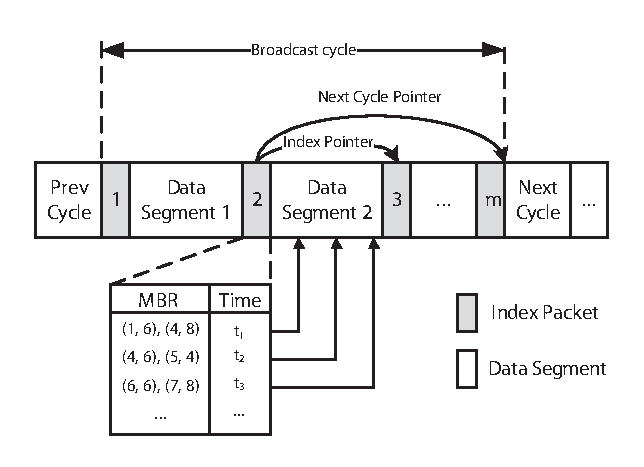
\includegraphics[width=3.5in]{Figures/index_packet.eps}
\caption{\small Broadcast program cycle format with index segments
and data segments.}
\label{fig:index_packet}
\end{center}
\end{figure}

%\begin{table}[h]
%\centering
%\begin{tabular}{l|l}
%  \hline
%  {\bf Attribute}   &   {\bf Description}\\
%  \hline
%  %\emph{data\_ptr}  &   Pointer to data packet\\
%  \emph{ind\_ptr}   &   Pointer to next index packet\\
%  \emph{bcast\_ptr} &   Pointer to beginning of next broadcast\\
%  \hline
%\end{tabular}
%\caption{Index Packet Attributes}
%\label{tab:index_attr}
%\end{table}

%Imielinski, et al in \cite{data_on_air} also included \emph{ind\_ptr}
%and \emph{bcast\_ptr} in data packet. We do not include these attributes
%in data packets to save bandwidth at the cost the initial index probe.
%Consider that a client tunes into the channel at a data packet. The client
%will have to keep tuning into the channel until the next index packet to
%get a ``road map" of the program. On average, the client would have to
%listen to half of the data segment, \(\frac{ds}{2}\), to get to the next
%index packet. Consider that a pointer of time takes $ptr$ of broadcast
%bandwidth. Let $bf$ be branching factor of an index tree. If we include
%both pointers in each data packet, additional bandwidth to include the
%pointers would be $2 \times ptr \times (bf^h + 1)$.

%A data packet does not contain any pointer, but contains multiple data
%records. $DataPacket$ = Header + $P$ $\subseteq$ $T$, where P is a set
%of tuples, and T is a set of tuples that consists of the entire data set.

%\begin{figure}[h]
%\begin{center}
%\line(1,0){240}
%\begin{verbatim}
%... Header ...
%Data Record       Attribute       Attribute
%Data Record       Attribute       Attribute
%Data Record       Attribute       Attribute
%...
%\end{verbatim}
%\line(1,0){240}
%\caption{\small Data Packet Format.
%\label{fig:data_packet_format}}
%\end{center}
%\end{figure}

%\subsection{Index Packing}
%
%For many tree index structures, including R-Tree, the branching factor
%of each node depends on the application. For a large data set, the
%branching factor would be larger than a smaller data set, to reduce
%height for the index, but the space utilization for each node would
%be higher.
%
%The space requirement to pack an index node
%into a broadcast packet depends on the branching factor of the tree.
%The number of entries in an index node equals to the branching factor.
%For example, for an R-Tree with branching factor of 4, space is
%required to store 4 MBRs and pointers.
%Since every entry contains a MBR and a pointer, larger the
%branching factor, larger the space requirement per node. The relationship
%is defined as follows:
%
%\begin{equation}
%s_n = b \times (s_{ptr} + s_b)
%\end{equation}
%
%Each index node can be packed into one index packet when the number of
%index entry is large. In this case the space utilization of each node
%before index replication is the space per node plus space of two
%pointers to the next index segment and broadcast cycle times the number
%of nodes in the index.
%
%\begin{equation}
%s_i = (b^{h} + 1) \times (s_n + 2 \times s_{ptr})
%\end{equation}
%
%If we pack multiple index nodes into one index packet, we can reduce
%the number of index pointers. In this case, if the next
%index node is in the same packet, we keep the same space utilization
%of a pointer but signify that the pointer to the next node is not a
%temporal, but instead a storage location within in this packet. The
%space utilization in this case is
%
%\begin{equation}
%s_i = \frac{b^{h} + 1}{n_p} \times (s_n + 2 \times s_{ptr})
%\end{equation}
%
%
%\begin{table}[h]
%\centering
%\begin{tabular}{c|l}
%  \hline
%  {\bf Notation} & {\bf Description}\\
%  \hline
%  $b$ & Branching factor of index tree.\\
%  $h$ & Height of index tree.\\
%  $s_{ptr}$ & Space utilization per pointer (ex: 16 bits).\\
%  $s_n$ & Space utilization per node.\\
%  $s_b$ & Space utilization per MBR.\\
%  $s_i$ & Total space of index tree.\\
%  $n_p$ & Nodes per packet.\\
%  \hline
%\end{tabular}
%\caption{Notations of packet format.}
%\label{tab:pf_notations}
%\end{table}

%\subsection{Motivation for DFDI}
%Consider that we have an R-Tree to index our multi-dimensional data, we
%need to consider the broadcast structure and format so that the index
%and data packets can be broadcasted on the same channel. Tree index
%structures are of particular interest since trees are non-linear whereas
%broadcast program is strictly linear. We consider two techiniques of
%embedding index as motivation for our index technique.
%
%One method is to embed the entire
%index tree at the beginning of the broadcast program as one big index
%segment (one huge packet or a series of continuous index packets). A
%drawback of this approach is that if the client misses the index segment,
%then no further processing can be done with the current cycle and the
%client has to wait for the next cycle. Another drawback is that the client
%have to download the entire index, although, the client may only be
%interested in a portion of the data. In addition, with our approach
%that the data packets do not have pointer to the next broadcast cycle or
%the next index segment, the client would not have a way to find out the
%time for the next cycle, except for continuously listening until the
%next cycle begins with new index.
%
%To mitigate the drawback, we could replicate and place the entire index
%segment of the previous method through out the broadcast program as
%proposed and discussed in \cite{data_on_air}. The drawback is that
%replicating the complete index several times increases
%the size of the broadcast program. For large data sets with large number
%of index nodes, this is inefficient.
%
%$\rightsquigarrow$ Consider an example that each pointer in an index packet is 16-bit
%(2 bytes). All 3 pointers takes 6 bytes.
%
%When coming in the middle of the program, a client really need an index
%packet, not the entire index, as a road map to when the next index
%will be available. This is the idea of the distributed index, in which
%the index is distributed in the program, but only a portion of the
%index is replicated.

\subsection{DFDI Allocation}

We have data indexed by a R-Tree. Our task now is to publish both
data and index on to the linear broadcast channel. DFDI allocates
space for index and data by performing a depth-first traversal of
the index tree as illustrated in Figure~\ref{fig:index_struct}. In
this process, the root index node $A$ is first included in the
cycle because it is first traversed. Index node $B_1$ is then
included in the program followed by $C_1$, then the data items
$D_1$ and $D_2$. One might argue that why use depth-first
traversal of the index tree, instead of breadth-first traversal
(BFT). The reason is that BFT would cluster all index into one
enormous index segment at the beginning of a cycle and basically
create a 1-time index.

DFDI replicate $L_r$ levels of the index tree $b$ times, where the
root node is considered level 1. Replication helps the clients get
a broader picture of upcoming broadcast items. When an index node
is replicated, only the MBRs that have no been broadcasted is
published; therefore the replication is \emph{not a complete
replication} of the node. Given $N$ to be the current node to be
published, if the level of $N$ is $L_r + 1$ or less, then the
parent of $N$ is replicated. Otherwise the parent is not
replicated.

An example is shown in Figure~\ref{fig:index_struct}, the root and
the B level index nodes are replicated. The replication helps the
client gets a broader picture of upcoming broadcast item. Of
course the best view would be to replicate the entire index, but
this would be the complete replication as discussed before and we
try to avoid to save broadcast bandwidth.
%Given two sibling index nodes $A$ and
%$B$ and their parent index node $P$, the following rules determine if
%an index node is replicated in the broadcast program:
%
%\begin{enumerate}
%\item If $A$ is the current index, and $P$ is part of the replicated
%        portion of the index, then $A.ind\_ptr$ points to an index packet
%        and segment that contains both $P$ and $B$.
%\item If $A$ is the current index, and $P$ is \emph{not} part of the
%        replicated portion of the index, then $A.ind\_ptr$ points to
%        an index packet (or segment) that contains only $B$.
%\end{enumerate}

\begin{figure}[h]
\begin{center}
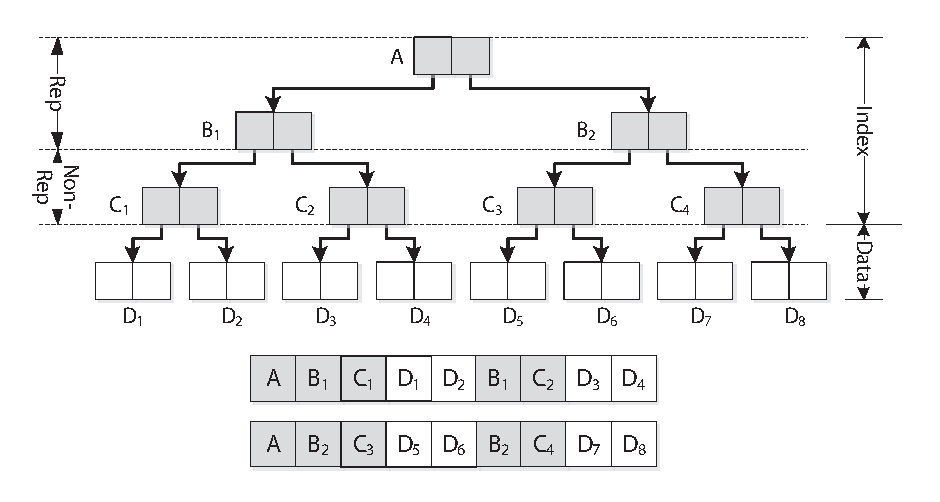
\includegraphics[width=3.5in]{Figures/bcast_struct.eps}
\caption{\small Index Structure. \label{fig:index_struct}}
\end{center}
\end{figure}

\begin{algorithm}
\algsetup{linenosize=\small,linenodelimiter=. }
\caption{DFDIPublish($Node$, $Level$, $L_r$)}
\label{alg:DFDIPublish}
\begin{algorithmic}[1]

\STATE PushToChannel($Node$) \COMMENT{Assume temporal ptrs are
known} \IF{$Node$ is Leaf}
    \FORALL{DataSegment in $Node$}
        \STATE PushToChannel(DataSegment)
    \ENDFOR
\ELSE
    \FORALL{ChildNode in $Node$}
        \STATE DFDIPublish(ChildNode, $Level$++)
        \IF{$L_r$ $\leq$ $L$ AND NOT Last ChildNode}
            \STATE PushToChannel($Node$)
            \COMMENT{Replication}
        \ENDIF
    \ENDFOR
\ENDIF
\end{algorithmic}
\end{algorithm}
%The space saving

%\subsection{Broadcast Structure}

%In this solution R-Tree is used to index data records. The records are presented geometrically in
%the R-Tree index as illustrated in Figure \ref{fig:skyline_mbr}, which shows the R-Tree representation of the records
%of Figure \ref{fig:data_records}. The R-Tree is not necessary used to index spatial data. Note that
%the reason R-Tree is used is because of its multi-dimension index capability and that we are able
%to multiplex multiple attributes in the same index. Almost
%any spatial index that supports space indexing will work with our approach. We choose R-Tree because its popularity
%nd support for high-dimensional data.

%As shown in Figure \ref{fig:skyline_mbr},  each axis of the Euclidean space represents a dimension
%(or attribute) in the dataset. For example, the x-axis represents the distance of the hotels from the beach
%and y-axis represents the price of the hotels. The records are inserted into an R-Tree as presented Figure \ref{fig:skyline_mbr}.

%\begin{figure}
%   \centering
%   \subfloat[Data records]{\label{fig:tablel}\includegraphics[width=1.5in]{table.eps}}
%   \subfloat[Data records inserted into R-Tree]{\label{fig:skyline_mbr}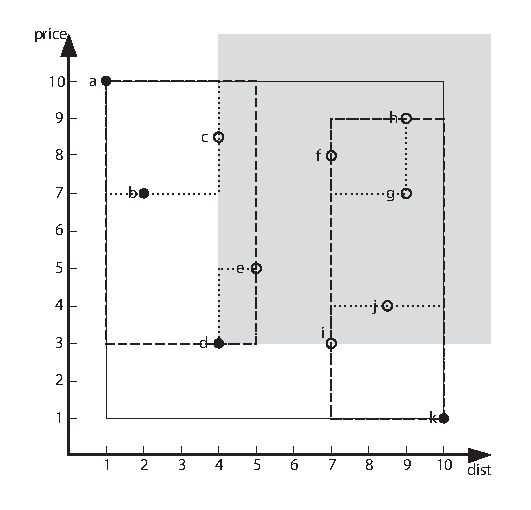
\includegraphics[width=1.5 in]{rtree_pr.eps}}
%   \caption{Data and R-Tree Index}
%   \label{fig:data_skyline_mbr}
%\end{figure}

%\begin{figure}[h]
%\begin{center}
%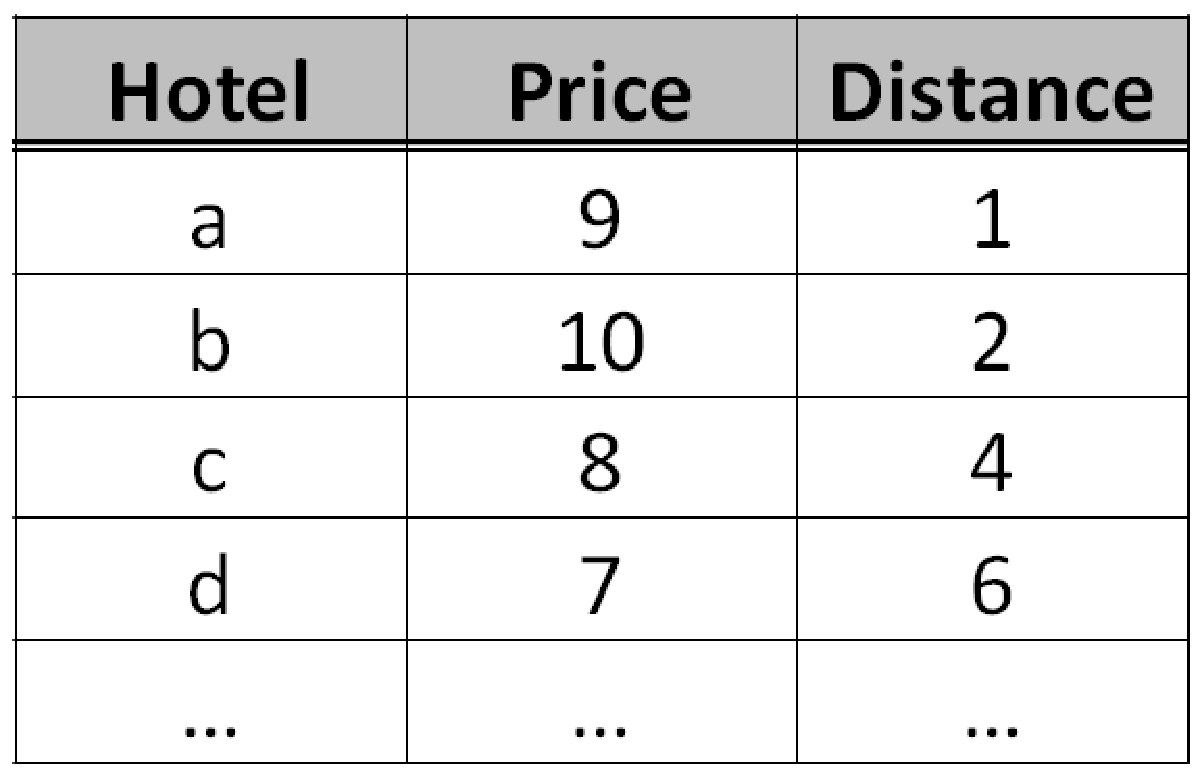
\includegraphics[width=2in]{Figures/table-eps-converted-to.pdf}
%\caption{\small Data Records.\label{fig:data_records}}
%\end{center}
%\end{figure}

%\begin{figure}[h]
%\begin{center}
%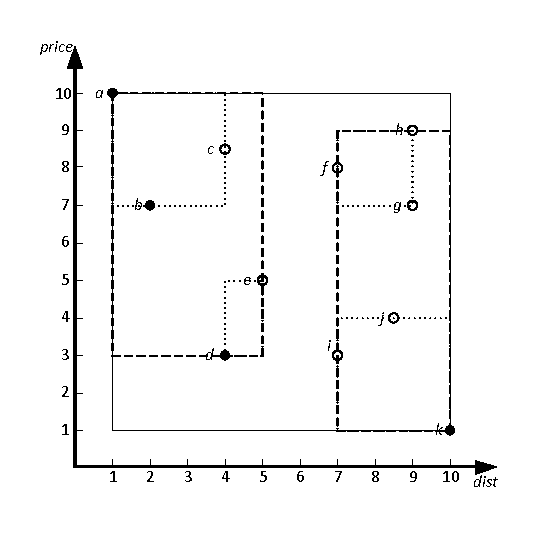
\includegraphics[width=3in]{Figures/rtree.pdf}
%\caption{\small Data Records inserted into R-Tree.\label{fig:skyline_mbr}}
%\end{center}
%\end{figure}

%The R-Tree index is multiplexed with the data records in the broadcast program using the distributed index technique as
%discussed in section \ref{sec:wireless_bcast_index} since the technique offers one of the best
%trade-off between broadcast space utilization and probing time for the client to find the first index packet.
%The broadcast program contains the intermingle of data packets and index packets as shown in Figure \ref{fig:bcast_cycle}.

%The index technique replicates upper levels of the index tree and does not
%replicate the lower portion (close to the leaves) of the index. The reason for only replicate a
%portion of the index is to conserve broadcast bandwidth while maintain the ability for the clients
%to recognize the state of the broadcast without waiting for the next cycle. The %replicated portion
%is broadcasted periodically, while non-replicated portion only broadcasted near the data item.

%The index packets are distributed amount the broadcast program, as in (1, m) index. The packets that contain replicated
%portion of the R-Tree index points to (the time of) the packets that contain non-replicated index. Similarly, the packets
%that contains non-replicated portion of the index eventually points to the data records. When we say point, or pointer,
%we mean an item, $p$, has the time of broadcast of another item $c$, denoted $p \to c$. See Figure \ref{fig:index_struct}.

\subsection{Analysis}

This section presents the efficiency analysis of our index design.
The efficiency metrics are defined in section 2.2.

\subsubsection{Index Percentage}

Index percentage measures the space overhead of the index
structure. It is defined to be the ratio between the space
allocated to index on the broadcast cycle to the length of the
entire broadcast cycle.

Let $L_r$ be the levels of replication (for example, $L_r$ for
Figure~\ref{fig:index_struct} is 2), $\eta$ be the space required
for an index node, and $\varepsilon$ be the space required for an
index node entry. The number of nodes replicated in the cycle is
$\displaystyle\sum\limits_{i=0}^{L_r-1} b^i$. For each replicated
node, the replication does not replicate the entire index node,
only the MBRs that has not been pushed to the channel; therefore,
additional space for each replicated node is
$\eta\displaystyle\sum\limits_{i=1}^{b-1} \frac{i}{b}$ or
$\varepsilon\displaystyle\sum\limits_{i=1}^{b-1} i$. The total
space taken by index is the space for each node, plus the
additional space for each replicated node and it is given by:

\begin{equation}
\iota = \eta(\displaystyle\sum\limits_{i=0}^{L_r-1} b^i
\displaystyle\sum\limits_{i=1}^{b-1} \frac{i}{b} +
\displaystyle\sum\limits_{i=0}^h b^h)
\end{equation}

Let $\theta$ be the size of the entire data set. The length of the
broadcast cycle is the space of the index plus the space of the
data:

\begin{equation}
\omega = \eta(\displaystyle\sum\limits_{i=0}^{L_r-1} b^i
\displaystyle\sum\limits_{i=1}^{b-1} \frac{i}{b} +
\displaystyle\sum\limits_{i=0}^h b^h) + \theta
\end{equation}

\subsubsection{Initial Index Prob}

The distributed index divides the entire data set into smaller
data segments and reduces the initial prob of first index segment.
The length of each data segment, denoted by $\varsigma$, is
determined by the number of index segments distributed among the
broadcast cycle. As one see from Figure~\ref{fig:index_struct},
there are four leaf-nodes and the data is divided into four
segments; therefore, the number of data segment is $b^h$ and size
per data segment is

\begin{equation}
\varsigma = \frac{\theta}{b^h}
\end{equation}

If we consider that the prob time is 0 when a client tunes in at
an index segment, then the expected initial index prob is the
average of length of each data segment:

\begin{equation}
E(\alpha) = \frac{2\theta}{b^h} = \frac{2\theta}{m}
\end{equation}

This is a big time reduction compare with one-time index prob.
